\section{MMTP Algorithm}
\label{sec:alg}

The MMTP algorithm  is described in detail in Refs.~\cite{brian,steve}. The trigger algorithm is summarized here,
mostly hilighting the adjustments needed to operate the algorithm with a cosmic muon detector.

The MMTP algorithm receives ADDC data and converts the ART addresses into Cartesian coordinates, look for subsets (``triggers'') which
 satisfy spatial and time prerequisites, and calculate quantities which carachterize these triggers.
 The first step is referred to as the \textit{decoder}, the second step is referred to as the \textit{finder},
 and the third step is referred to as the \textit{fitter}.
 The present MMTP is firmware is synthetized and run on a Xilinx Virtex-7 FPGA in a VC707 evaluation board.
 

\subsection{Decoding}
\label{sec:alg-decode}

 The MMTP converts the VMM and strip numbers into Cartesian coordinates 
 taking into consideration that some of the MM chambers are flipped relative to each other.
 The MMTP measures coordinates in units of strip pitch (400$\mu$).
 For example, if   strip 30 in VMM 5 is  converted into  a position 
 $x=$ 350 = $5*64 + 30$. 
The first octuplet board (board 0 in Fig.~\ref{fig:cartoon_road_demo})  is set at $Z=0$, and the following boards at their respective distance measured in pitch
 units.
% The MMTP then adds the distance from the beamline to the base of the MM chamber, in units of strips, to the global strip number, 
%and divides the global strip number by the $z$-position of the chamber, to convert the strip to a slope, $x_\text{strip} / z_\text{strip}$.

\subsection{Finder}
\label{sec:alg-finder}
The next step of the MMTP algorithm is to search the data of all boards (at different $z$ positions)
for hits in a given time and $x$ window consistent with a straight track with angle of incidence smaller than 25$\deg$.
 This step is called the \textit{finder}.

The finder assigns hits in each board to 8 $X$-roads (1 VMM or 64 strips or 25.4 cm wide), and evaluates
simultaneously if any road contains enough hits to generate a trigger.
A road must contain at least two hits on the $X$ planes and at least two hits on the stereo ($UV$) planes to generate a trigger.
 Additionally, at least two of the hits on $X$-planes must occur on different quadruplets, to ensure a good slope resolution when
 later  fitting the $X$-hits with a straight line.
 These requirements are looser than those ($3X$ AND $3UV$)  anticipated in the
  NSW TDR to compensate for the MMFE8 board inefficiencies caused by the increasing number  of VMM channels zapped by the
 Micromegas  high voltage~\cite{noiseless}.
 A graphic visualitation of the finder algorithm is shown in Fig.~\ref{fig:cartoon_road_demo}.

\begin{figure}[!htpb]
  \begin{center}
    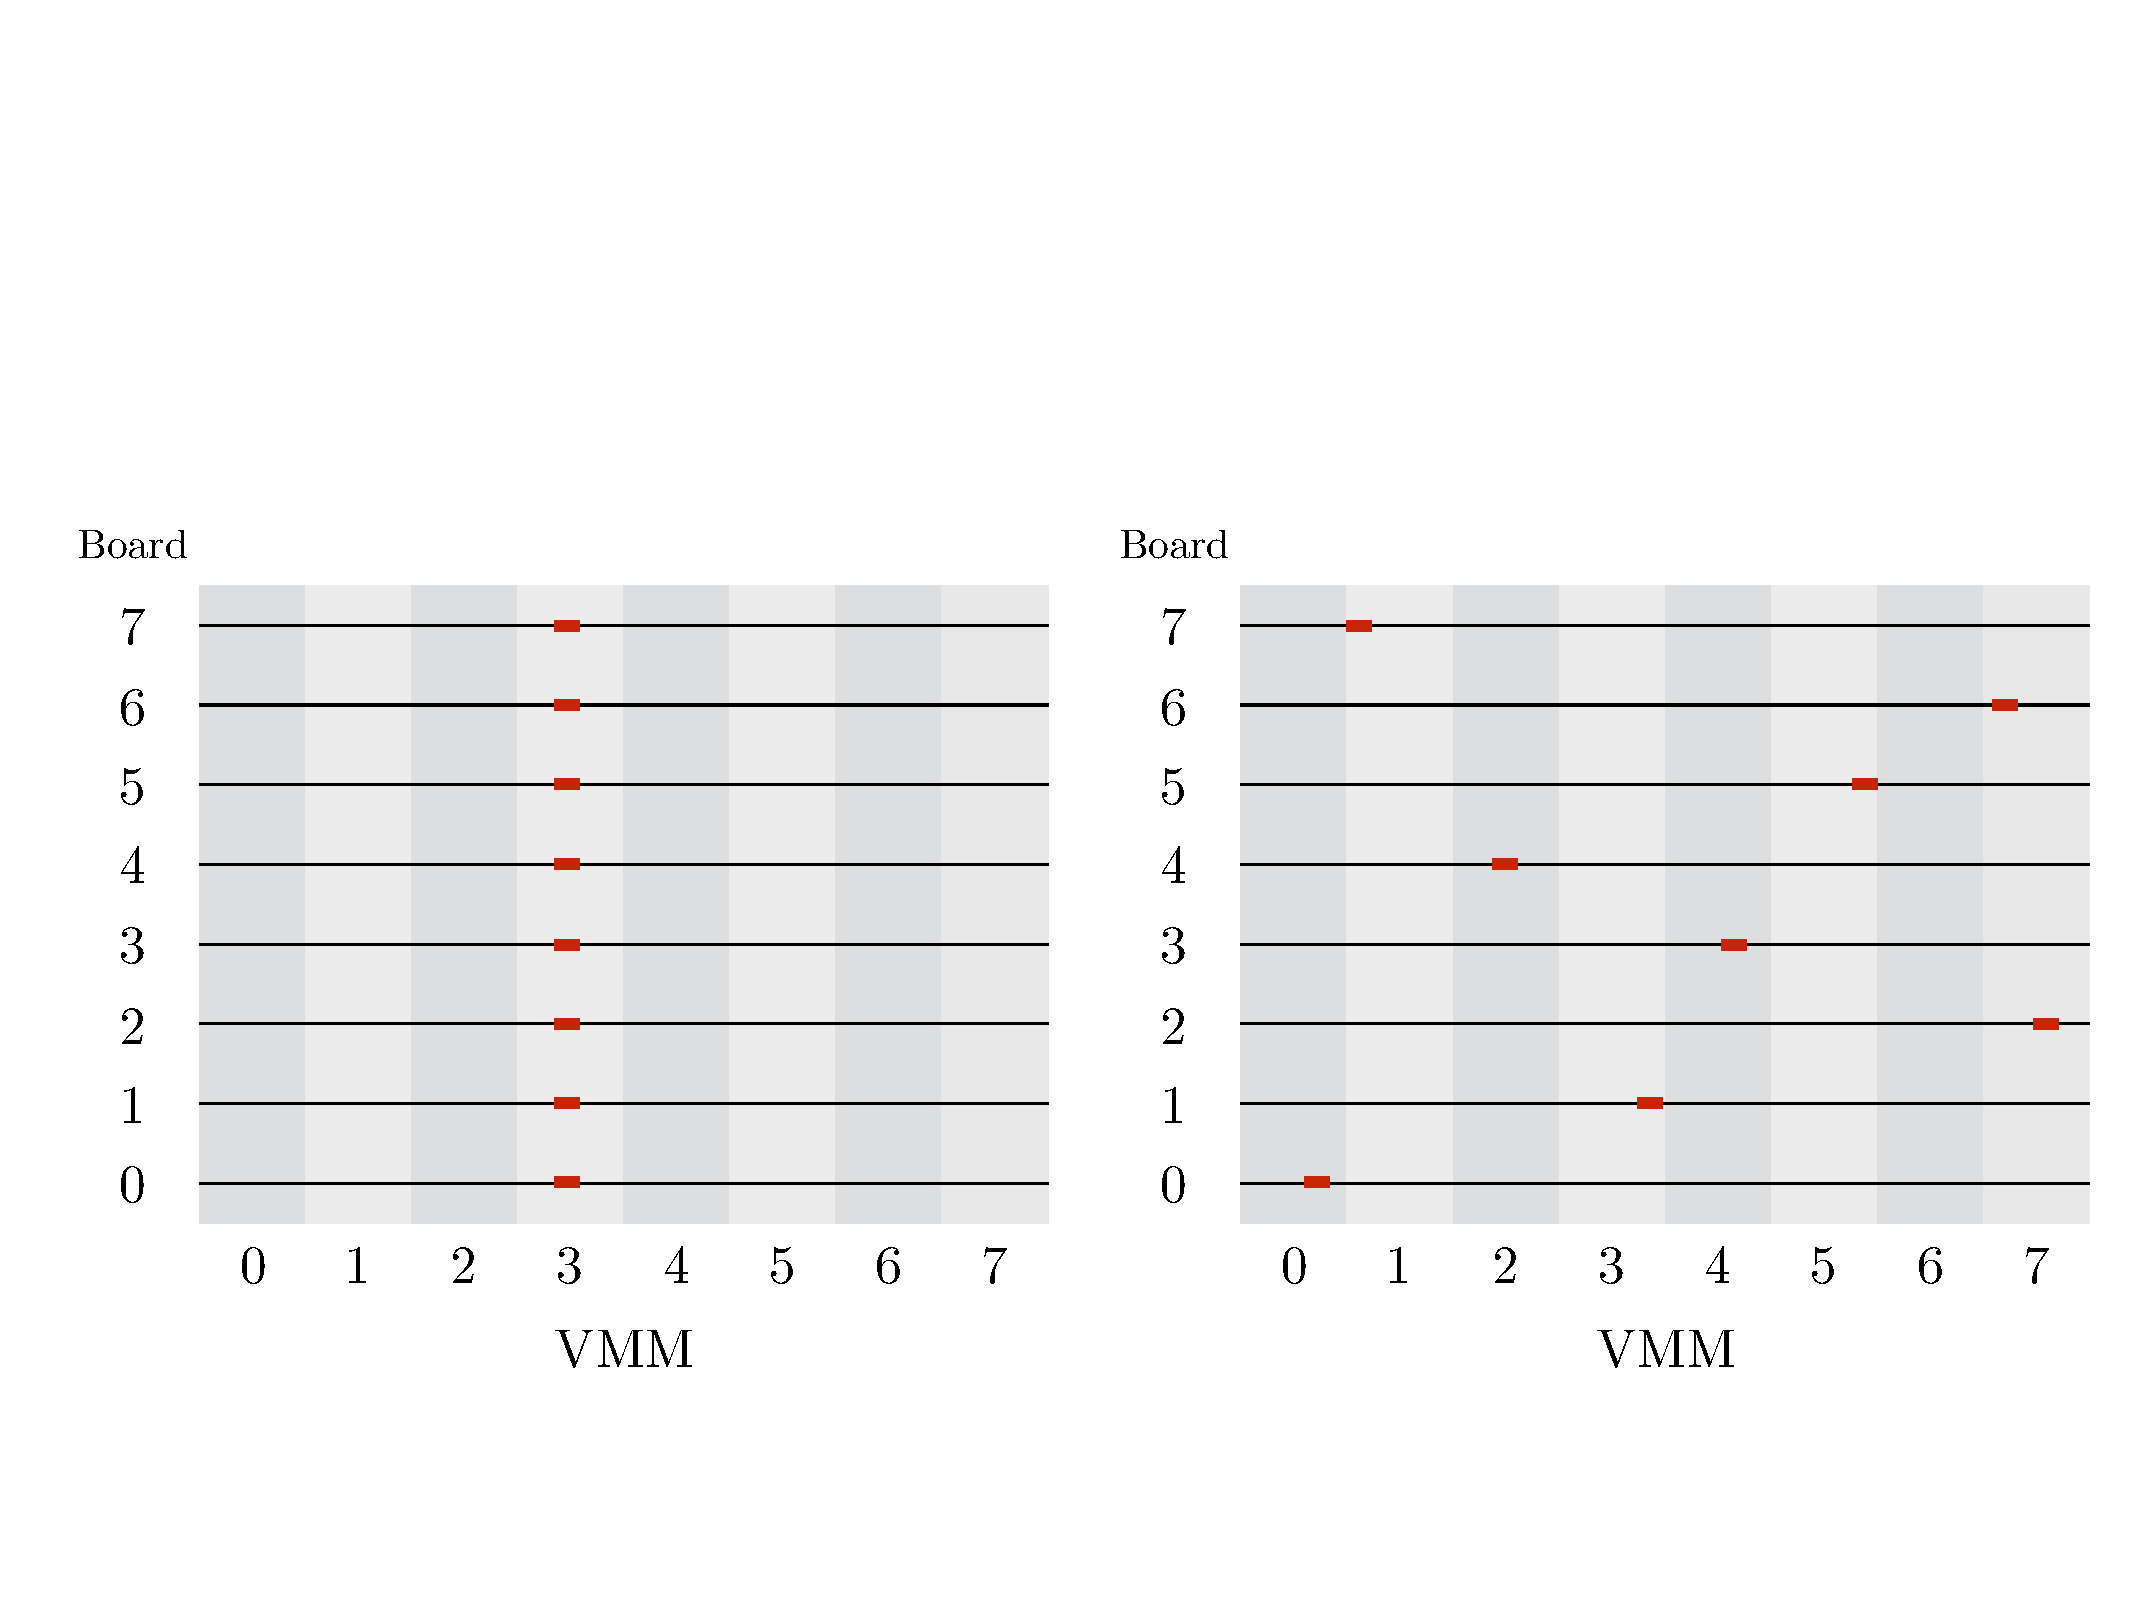
\includegraphics[width=1.0\textwidth]{figures/cartoons/cartoon_road_demo}
  \end{center}
  \vspace{-20pt}
  \caption{Hits generated by a cosmic muon passing through the octuplet (left) and
  randomly generated (right) as seen by the finder algorithm. Roads are 1-VMM wide and shown in alternating gray colors.
 Only the event on the left would generate a trigger.}
  \label{fig:cartoon_road_demo}
\end{figure}

To recover those  cases in which a muon with a large angle of incidence deposits hots in two different roads, 
 the finder algorithm seareching as road also uses hits  in the 2 neighbor roads. 
 For example, road 3 uses hits from VMM 2, VMM 3, and VMM 4, so that the effective road size is 3 VMMs.
 The  angle of incidence cosmic muons collected by our telescope can be as large as 25$\deg$~\cite{noiseless}
 and is well covered with  an effective road size of 3 VMMs.

The finder also requires candidate hits to lie within a given time window in units of the BC clock.
Based on previous measurements of the time jitter of ART signal~\cite{ }, we chose to start with a 7 BC window~\footnote{Due to a bug in 
the MMTP firmware, this window is sometimes 8 BCs in Run 3522. The bug was corrected prior to Runs 3527-3530. Runs are discussed 
in more detail in Section~\ref{sec:data-taking}.}.
 The time window is implemented as follows. A board hit in a given road is stored  for seven BCs.
 No new hits are allowed in that road and that board until the hit is ``old'', i.e., after seven BCs.
 As new hits are entering into other boards, the trigger requirements are evaluated for all roads in parallel. 
 If a trigger was found in a road,
 a trigger is issued when the earliest hit in the road becomes ``old''. That trigger carries the BCID of the ``old'' hit.

Each road can provide  one trigger per cycle of the BC clock. The triggers
 found  in all roads with the same BCID are placed in a road-number-based priority encoder  and sent sequentially to the fitter for further calculations.
 Because the MMTP clock is eight times faster than the BC clock, almost no issued trigger is lost.

\subsection{Fitter}
\label{sec:alg-fitter}

The  \textit{fitter} algorithm  provides the location and quality of a trigger.
The location is represented by a point in the  $\eta-\phi$ space which in the NSW upgrade is used by downstream
trigger modules to define the L1 muon trigger region of interest (ROI). 
The algorithm a fits the finder hits with a straight line without  (\textit{local}) and with ( \textit{global})
 the constraint that the straight line originates from the interaction point.
 A cut on the slope difference  $\Delta\theta = |\theta_g - theta_l |$ is supposed to reduce the rate of accidental triggers.

In ATLAS, the global slopes are calculated as  $m_l= <x_l/z_l> $. For each hit
  measured by $l=X$ or $l=U$ or $l=V$ planes, the value $x_l/z_l$ , where $x_l$ is the value of the precision coordinate
 and $z_l$ is the  distance  from the interaction point ($\simeq$750 cm), is returned by look-up-tables (LUT).
The 3 slopes are converted with look up tables which first 
 return  $m_y=\frac{m_U - m_V}{2\ \text{tan}(\theta_\text{stereo})}$ and $\eta$, $\phi$ coordinates from the $m_x,m_y$ values.


Since cosmic muons do not originate from a point-like source, the fitter algorithm has been modified to use strip numbers instead of slopes
(we use a new LUT which does not divide $x$ by the distance from the interaction point).
The local slope is evaluated as    $m_x^\text{local} = \sum c_i \ x_i$, where the sum includes all $X$ hits, and $c_i$ are constants,
stored in a new LUT, which depend on the $z$ position of the $X$ plane (see Table~1) in units of strip pitch. 
 The detector distance from the beamline is set to 0.
 Instead of the global slope, we evaluate <x_l> and <z_l> for all  $X,U,V$ hits separately.

 In addition, the MMTP algorithm stores: a) the ADDC data in 15 BC preceeding the trigger BCID; b) the trigger BCID, the address of the hits
 providing a trigger, the local slope, and other ancillary information; c) the BCID of a scintillator trigger into 3 different FIFO,
 the content of which is transmitted as UDP packets
 in round-robin mode and recorded.
 
\subsection{Method for evaluating the MMTP spatial resolution}
\label{sec:alg-resol}

 We check the MTTP performance by using events in which we reconstruct a track using Micromegas clusters.
 The cluster selection is described in Ref.~\cite{noise}. In particular, the  BCID of the hits forming a cluster is required
 to be in a 15 BC windows around the BCID of the scintillator trigger.
 As explained in Ref.~\cite{noisy} we fit the available cluster with two straight lines in the $x-z$ and $y-z$ planes.
 The fits, referred to as MM, are done in the same coordinate system as the MMTP. The fits provide slopes, $M_X$ and $M_Y$, and intercepts, $A_X$ and $A_Y$
 which are used to set limits to the MMTP space resolution. In the assumption that the uncertainty of the parameters returned by MM fits 
  are negligible,  comparisons with MMTP results measure its accuracy.

  We SELECT tracks the clusterS of which satisfy the trigger requirements. The number of MMTP triggers found in the latter
 set measures the MMTP efficiency.

 To measure the resolution we compare the MMTP <x_X>  to  $A_X$+ $M_X$ <z_X>. The rms value of their difference divided by 750 cm
 yield the $m_x$ resolution.
 We also evaluate the MMTP accuracy in measuring the $y$ coordinate. We extrapolate the  <x_U>, <x_V>, <x_V> values calculated
 using the trigger hits to a coomon $z$ value using the result of the MM fit. At that $z$, we evaluate $y_{\rm TP}$
 as   $\frac{x_U - x_V}{2\ \text{tan}(\theta_\text{stereo})}$ or  $\frac{x_X - x_V(U)}{\ \text{tan}(\theta_\text{stereo})}$.
 These values are compared to  $y_{\rm MM}$ derived from the MM fit at the same $z$.
 

  




 One is the $\phi$ angle determined from 
 The fitter presently does not create or remove any triggers. The final implementation of the MMTP algorithm may include a quality requirement
 from the fitter, namely $\Delta\theta < 15^\circ$.

For the NSW upgrade, the main deliverables of the fitter are the location and quality of a trigger. 
The location is represented by a region of interest (ROI), which is a number provided by downstream clients like
 Sector Logic mapping to $\eta-\phi$ space. The quality of the trigger is represented by the difference in angle
 a \textit{local} fit of the trigger ART hits and a \textit{global} fit. A \textit{local} fit is performed
 on only the ART hits, and a \textit{global} fit is performed with the constraint that the trigger be consistent
 with the interaction point. The difference is called $\Delta\theta$.

The location of the trigger is derived in a Cartesian $m_x-m_y$ space, where $\hat{y}$ points perpendicular to the direction
 of the $X$-strips, $\hat{x}$ points parallel to the $X$-strips, and $m_i$ is the slope $i/z$. $m_y$ is measured as 
the average of slopes measured in each $X$-plane, $\overline{m_X}$. $m_x$ is measured as the difference
 between slopes measured in the $U$ and $V$ planes, with a geometric factor from the angle of the
 stereo strips: $\frac{m_U - m_V}{2\ \text{tan}(\theta_\text{stereo})}$. The standard ATLAS coordinates
 $\eta$, $\phi$ can be derived directly from $m_x$, $m_y$, where the resolution of $\eta$ ($\phi$) is dominated by
 the resolution of $m_y$ ($m_x$). Rather than calculate $\eta$, $\phi$, however, the slopes $m_i$ are sent as an address
 to a LUT which returns a ROI.\footnote{We apologize for the confusing notation. 
To recap: $X$, $U$, and $V$ denote different layers of Micromegas. $x$, $y$, and $z$ are cartesian coordinates. 
The $X$-layers measure $m_X$, which is used to derive $m_y$. And so on.}

To calculate the quality of a trigger, the fitter compares the slopes of a linear fit of the ART data with and without a
 constraint that it originate at the interaction point. These are referred to as \textit{global} and \textit{local} slopes, 
respectively, and they only use hits from the $X$-planes. The global slope is simply the aforementioned $m_y$, or $\overline{m_X}$. 
The local slope is calculated as $m_x^\text{local} = \sum c_i \ y_i$, where the sum includes all $X$ hits, $c_i$ is a constant depending
 on which $X$-planes are used in the fit, and $y_i$ is the position of the hit. $c_i$ is stored in a LUT,
 and the multiplication/addition is performed by the FPGA. This analytic ``fit'' gives the slope of
 the least-squares line, and is more appealing than an iterative fit given the hardware constraints.
 The difference in angles $\Delta\theta$ can be calculated directly from $m_x^\text{local}$, $m_x^\text{global}$, but instead these
 slopes are sent as an address to a LUT which returns $\Delta\theta$.

\subsection{Output}
\label{sec:alg-output}

The MMTP will send its triggers to the sTGC trigger processor FPGA, where duplicates will be discarded before being sent to downstream clients.
 The NSW TP in total will send at most 8 triggers per BC per sector. Each trigger will be composed of 24 bits,
 and presently the bits are allocated as 5 bits for $\Delta\theta$; 5 bits for $\phi$ ROI; 8 bits for $\theta$ ROI; and 6 spare bits.

\subsection{Adjustments for cosmic muons}
\label{sec:alg-crts}

The use of \textit{slopes} instead of \textit{strips} in the algorithm is motivated by the knowledge that particles arriving at the NSW from a proton-proton
 collision should travel in a nearly straight line. Thus, each layer of MM will record a different strip address for the incident particle,
 but a nearly identical slope. This simplifies logic for defining spatial \textit{slope-roads} in the MM chamber.

However, for a cosmic ray test stand, the exact origin of incident particles is unknown.
 The MMTP algorithm is then modified to use strip addresses instead of slopes for the defintion of roads,
 as discussed in Section~\ref{sec:alg-finder}. The implementation of strip-to-slope conversion in the FPGA is
 nonetheless tested by multiplying each strip address by 1, instead of $1/z_\text{strip}$, 
to calculate a ``slope'' which is suitable for spatial coincidences of cosmic muons. 
Using strips instead of slopes is the largest conceptual difference between the ATLAS implementation and the cosmic 
muon implementation of the algorithm, and it will be relevant for the analysis in Section~\ref{sec:perf}.

Additional adjustments to the MMTP algorithm for use at the cosmic ray test stand include:

\begin{itemize}
  \item The overall chamber offset from the beamline is removed, though the machinery of adjusting the overall offset is kept
  \item Plane-specific offsets from the beamline are essentially removed, though the machinery of adjusting the global strip is kept
  \item The number of neighboring roads considered for each road in the finder is 2 for $X$ and $UV$ planes, whereas for ATLAS it is 2 (5) for $X$ ($UV$)
  \item The constants $c_i$ of the local slope calculation depend on the geometry of the octuplet, and are adjusted for the mini-octuplet
  \item Offline, the precision coordinate of the MMTP is referred to as $x$, and the non-precision coordinate is $y$,
 because we found it confusing otherwise
\end{itemize}

Finally, the MMTP algorithm stores copies of the input ART data and output trigger data in FIFO buffers,
 which are transmitted as UDP packets via ethernet to a computer for analysis.

% \subsection{Bugs encountered}
% \label{sec:alg-bugs}
%
% By January 2017, the MMTP algorithm had been implemented in firmware and successfully created triggers in behavioral simulation. By summer 2017, the MMTP algorithm is implemented on a FPGA and records hundreds of thousands of cosmic muon triggers per day. Many bugs were uncovered along the way.
%
% \textbf{Put some bugs here.}

